\section{Metodologia}

\subsection{Fases do Projeto}
O primeiro passo do projeto foi demarcado com a definição do tema, que teve origem em conversas com o professor Dr.André Luis Meneses Silva e em pesquisas realizadas. Após essa fase, iniciamos uma pesquisa e estudos acerca da plataforma \href{https://wokwi.com/}{Wokwi}, para a implementação dos módulos e códigos utilizados na \textit{Raspberry Pi}, para a lacração, limpeza da lixeira e futuramente da \textit{Inteligência artificial} (paralelo ao desenvolvimento, será feito a escrita no TCC 2) para a separação automática do lixo. Após isso, foi feita a pesquisa de trabalhos relacionados na área da modelagem de \textit{hardware} e \textit{software}. E então, foi feito um levantamento bibliográfico sobre os assuntos relacionados ao projeto como: IoT, microcontroladores, sensores, atuadores,  microcomputadores e inteligência artificial.

O segundo passo foi a análise de custo de construção e instalação da lixeira, ao qual foram analisados diversos módulos, porém apenas selecionados os que formassem um conjunto de aparelhos que realizassem o esperado e de forma barateada, melhorando o custo benefício de aquisição da lixeira. Por fim, será encaixado os aparelhos nos devidos locais, valendo ressaltar que a \textit{válvula solenóide} de escoamento deve ser implantada na parte de baixo para gerar um efeito centrífuga na água, e a de bombeamento na parte lateral para melhorar a eficiência da limpeza.

\subsection{Implementação do Projeto}
Para com a implementação e design do projeto usamos uma raspberry pi, que será usada para controlar os dados de leitura dos 2 (dois) HC-SR04, que serão instalados uma na camada inferior da parte de dentro da tampa, e outra na camada superior da parte de dentro da base da lixeira, ao qual a primeira servirá com o intuito de verificar o quão cheia está a sacola de lixo, e assim que verificado que está cheia o servo motor irá operar o mecanismo de amarração de fita à sacola de lixo. Já a segunda HC-SR04, servirá com o intuito de verificar a existência de uma sacola. Atrelado a raspberry pi terá também uma bomba de água, que irá receber o sinal da segunda HC-SR04, fazendo ou não o bombeamento da água ligado diretamente a encanação, a qual puxará a água diretamente da fonte, e fará o descarte da água residual no esgoto por meio das encanações. Isto, utilizando de 2 (duas) válvulas solenoides, para controlar o fluxo de água passada pela bomba de água, a primeira será utilizada com o intuito de abertura para o enchimento de água na lixeira, já a segunda para o esvaziamento da água contaminada.

\subsection{Recursos}
Os recursos que serão utilizados para o desenvolvimento do projeto estão relacionados ao hardware necessário e ao ambiente de desenvolvimento de código. O hardware necessário será dois microcontroladores HC-SR04 que foram apresentados na Figura \ref{fig:sensor}, um servo motor que foi apresentado na Figura \ref{fig:servomotor}, duas válvula solenóide que foram apresentadas na Figura \ref{fig:válvula selenóide}, uma bomba de água que foi apresentada na Figura \ref{fig:bomba}, os quais serão acoplados a uma Raspberry pi. Fora a necessidade da ligação as tubulações para a limpeza e descarte da água residual, além de uma polia para realizar a rotação do servo motor com a fita.

\subsection{Avaliação do Impacto Social}
Como avaliação do impacto social, é analisado sobre como a lixeira inteligente irá impactar no âmbito social, na boa relação entre os grandes centros urbanos e o meio ambiente e em como a falta do tratamento devido traz à tona prejuízos para todos os seres vivos e não vivos. 

A priori, a redução do mau odor das lixeiras é uma medida fundamental para melhorar a qualidade de vida e o bem-estar das pessoas, bem como para minimizar os impactos negativos nos animais que vivem nas proximidades. Além da limpeza constante, o uso de sacos de lixo resistentes e à prova de vazamentos pode ajudar a conter os odores desagradáveis provenientes da mistura de materiais orgânicos e inorgânicos. Outra estratégia eficaz envolve o armazenamento adequado dos resíduos, como o uso de recipientes herméticos, que evitam a disseminação dos odores. Essas práticas não apenas reduzem o mau odor, mas também contribuem para manter a higiene e a saúde das comunidades, criando um ambiente mais agradável e saudável para todos. Além disso, ao minimizar o mau odor, reduz-se o risco de atração de pragas, como insetos e roedores, que podem representar problemas adicionais de saúde e segurança. Portanto, o cuidado com a gestão de resíduos e a mitigação dos odores desagradáveis são aspectos cruciais do gerenciamento de resíduos em áreas urbanas e rurais.

A posteriori, surge a necessidade de lidar com a secreção causada pela falta da higienização adequada aos lixos, que é o chorume. Tal líquido é tanto nocivo para os seres vivos que entram em contato, quanto para com a contaminação de lençóis freáticos e poços artesianos nos centros urbanos. Em relação aos animais, que entram em contato com líquido tóxico que se forma a partir da decomposição de resíduos orgânicos, sofrem com o  envenenamento. Além disso, o vazamento de chorume pode contaminar o solo e as fontes de água próximas, destruindo habitats naturais e tornando esses ambientes inadequados para a vida selvagem. Já em relação aos humanos, a contaminação do chorume nos lençóis freáticos e poços artesianos representa uma séria ameaça à qualidade da água potável. O chorume, ao infiltrar-se nessas fontes subterrâneas, pode poluir a água com substâncias tóxicas, tornando-a inadequada para consumo humano. Isso coloca em risco a saúde.

\subsection{Detalhamento}
 \begin{figure}[H]
    \caption{Imagem do Circuito do projeto}
    \label{fig:sensor}
    \begin{center}
        
        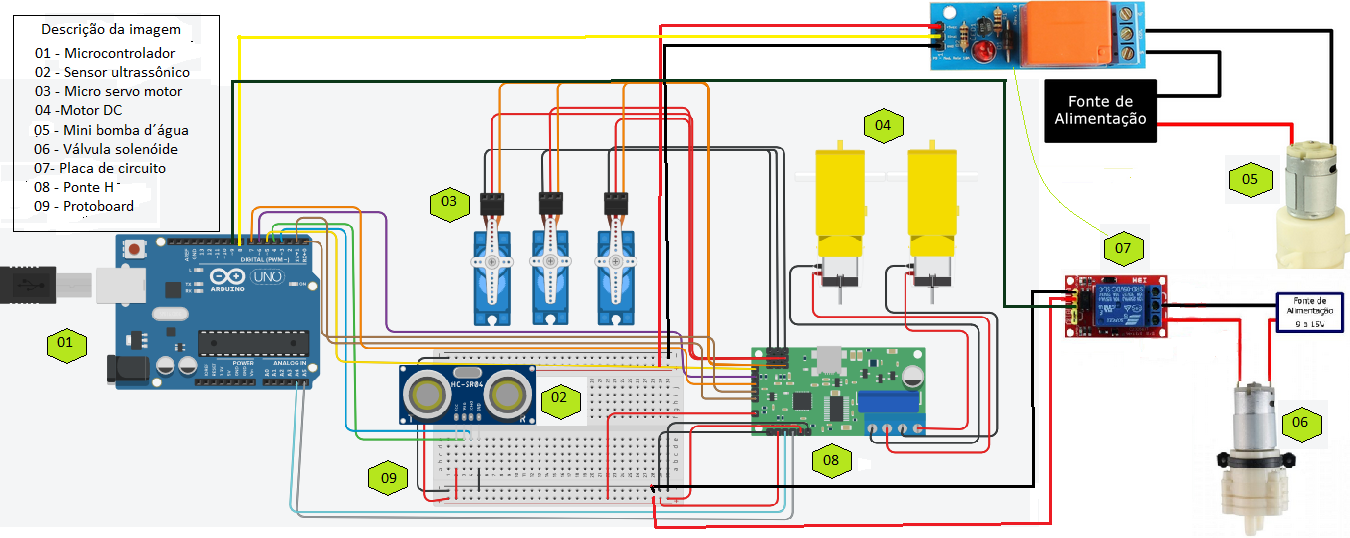
\includegraphics[scale=0.5]{circuito.png}
        
        Fonte: Autoria própria
    \end{center}
\end{figure}

A Figura 6 é um pequeno esboço do projeto, numa visão do hardware que o compõe e suas conexões. Na criação dessa figura foi utilizado o software Thinkercad e posteriormente editada a imagem no paint. Na imagem temos Arduino que fará o papel de microcontrolador, também temos três micro servos motores e dois motores DC ligados a uma ponte h que está conectada ao Arduino. Temos também uma bomba d'água ligadas numa placa de circuito que está conectada ao Arduino e uma válvula solenoide ligada a uma placa de circuito e conectada ao Arduino.

A lixeira irá possuir na frente um painel, nesse caso, um tablet para usuário informar qual o lixo que deseja descartar. Após o usuário informar qual o tipo de lixo ele deseja descartar a lixeira se abre e a tela solicita que o usuário deposite o lixo especificado.

Dentro da lixeira há um desnível controlado por um motor que ao ser colocado o lixo ele abre o compartimento respectivo para o descarte desse lixo. Dentro do compartimento há um sensor ultrassônico na parte superior, um motor para inserir a sacola de lixo nova e lacrar a sacola de lixo cheia sempre que necessário, embaixo há um sensor de peso acoplado a uma esteira que ao alcançar o peso especificado no projeto que irá informar ao sistema que o lixo está cheio na parte inferior traseira interna de cada compartimento há um motor acoplado há uma saída por onde o saco de lixo lacrado será enviado pela esteira para um compartimento onde estará disponível para coleta e reciclagem. Para facilitar a coleta, o saco de lixo em cada compartimento deverá ter uma cor diferente de acordo com as especificações de coleta e reciclagem e assim facilitará o trabalho do coletor.

Nos compartimentos necessários, onde há materiais orgânicos e materiais que possam ser reciclados porém sujos ou que necessitam de um pré-processamento, haverá nas laterais um motor acoplado a uma bomba d'água com o mecanismo de alto limpeza evitando o mau odor do lixo e abaixo destes compartimentos teremos uma válvula solenóide na saída por onde a água suja irá por encanamento para o esgoto evitando assim a contaminação do solo.







